\documentclass[11pt, a4paper]{article}

% --- 1. LANGUAGE & ENCODING ---
\usepackage[utf8]{inputenc}
\usepackage[T1]{fontenc}
\usepackage[english]{babel}

\usepackage{geometry}
\geometry{left=2.5cm, right=2.5cm, top=2.5cm, bottom=2.5cm}

% --- 2. FONTS & MATH ---
\usepackage{amsmath, amsfonts, amsthm}
\usepackage{newtxtext, newtxmath} % Times font

% --- 3. GRAPHICS, PLOTS & TABLES ---
\usepackage{graphicx}
\usepackage{float}
\usepackage{pgfplots}
\usepackage{tabularx}
\usepackage{booktabs}
\usepackage{xcolor}
\pgfplotsset{compat=1.18}
\usetikzlibrary{arrows.meta, decorations.pathmorphing}

% --- 4. FORMATTING ---
\usepackage{ragged2e}
\usepackage{microtype}
\usepackage{setspace}
\linespread{1.05}

% --- 5. AUTHOR & LINKS ---
\usepackage{authblk}
\usepackage[colorlinks=true, allcolors=blue, pdfencoding=auto, hypertexnames=false]{hyperref}

% --- 6. THEOREM ENVIRONMENTS ---
\newtheorem{definition}{Definition}
\newtheorem{proposition}{Proposition}
\newtheorem{theorem}{Theorem}
\newtheorem{hypothesis}{Hypothesis}

% --- 7. METADATA ---
\title{\texorpdfstring{\textbf{Toward a Topological Paradigm of Compute: \\ Isomorphism Between LLM Reasoning Manifolds and Quantum Correlation Structures}}{Toward a Topological Paradigm of Compute: Isomorphism Between LLM Reasoning Manifolds and Quantum Correlation Structures}}
\author{\textbf{Dang, Van Truong}}
\affil{Independent Researcher \\ Ho Chi Minh City, Vietnam \\ \texttt{ks.dangvantruong@gmail.com}}
\date{\today}

\begin{document}

\maketitle

% --- ABSTRACT ---
\begin{abstract}
\noindent Recent findings in large language models (LLMs) reveal that effective long chain-of-thought (Long CoT) reasoning trajectories form stable ``molecular'' structures, characterized by covalent-like deep reasoning, hydrogen-like self-reflection, and van der Waals-like exploration \cite{chen2026}. We argue that this emergence of topological organization implies that while the hardware remains classical, the semantic interactions in high-dimensional space exhibit quantum-like behaviors.

In this perspective, we introduce the \textbf{Correlation-Aware Programming Model (CAPM)}, a theoretical framework that abstracts quantum computation via an Entanglement Resource Graph (ERG). We formalize a structural isomorphism between the AI reasoning manifold ($G_{AI}$) and the quantum resource graph ($G_{Q}$), specifically leveraging \textit{Tensor Networks} and \textit{Measurement-Based Quantum Computing (MBQC)} principles \cite{nielsen2010, levine2021}.

We posit that true quantum advantage in reasoning stems from \textit{topological resonance}---a mechanism where the Attention Mechanism simulates quantum non-locality to bypass energy barriers. This framework offers a unified blueprint where Entropy Convergence in AI aligns with Ground State Cooling in quantum systems.

\vspace{0.3cm}
\noindent \textbf{Keywords:} Chain-of-Thought, Tensor Networks, Entanglement Resource Graph, Topological Isomorphism, CAPM, Quantum-AI Convergence, Cluster States.
\end{abstract}

% --- 1. INTRODUCTION ---
\section{Introduction}
Both large language models (LLMs) and quantum computing architectures are confronting fundamental barriers to scaling. In LLMs, reasoning often fails to emerge robustly due to error propagation in linear chains. Similarly, gate-based quantum systems suffer from the ``decoherence wall'' in noisy intermediate-scale quantum (NISQ) devices \cite{nielsen2010}.

These parallel challenges expose a shared limitation: traditional approaches treat computation as a sequence of local operations, failing to exploit global topology. Recent work by Chen et al. (2026) offers a transformative insight: effective reasoning emerges not from linear chains, but from folded, molecular-like structures \cite{chen2026}.

% --- DISCLAIMER ---
\begin{center}
\fbox{
\begin{minipage}{0.9\textwidth}
\textbf{Disclaimer on Physicality vs. Isomorphism:}
It is crucial to clarify that we do not imply LLMs utilize physical quantum effects (such as superposition of hardware states) within the silicon chips. Rather, we posit that the \textit{mathematical topology} of the reasoning manifold in high-dimensional vector space behaves isomorphically to quantum graph states. From this perspective, an LLM acts as a classical engine simulating an effective semantic quantum field theory, where phenomena like semantic entanglement and interference naturally emerge from massive parameter interactions.
\end{minipage}
}
\end{center}

In this paper, we introduce the \textbf{Correlation-Aware Programming Model (CAPM)}, reorienting quantum computation toward explicit management of correlation topology via an Entanglement Resource Graph (ERG). We demonstrate how the ``folding'' in AI serves as the algorithmic equivalent of ``quantum tunneling'' in hardware.

% --- 2. RELATED WORK ---
\section{Related Work}

\subsection{From Linear Chains to Molecular Manifolds}
The breakthrough by Chen et al. (2026) identifies the ``Molecular Structure of Thought,'' demonstrating that reasoning behaviors map to chemical bonds: \textit{Deep Reasoning} (covalent), \textit{Self-Reflection} (hydrogen), and \textit{Self-Exploration} (van der Waals). They establish a link between Attention weights ($\alpha_{ij}$) and Gibbs-Boltzmann energy, bridging statistical physics and cognition \cite{chen2026}.

\subsection{Tensor Networks: The Bridge Between AI and Quantum}
A key theoretical foundation for our isomorphism is the connection between Transformer architectures and Tensor Networks (TN). Physicists use TNs (e.g., Matrix Product States - MPS, PEPS) to simulate quantum many-body systems on classical computers. Recent studies suggest that the Transformer architecture is mathematically equivalent to a trainable Tensor Network, capable of capturing long-range correlations and entanglement-like structures in data \cite{levine2021, gao2022}.

% --- 3. THE ISOMORPHISM HYPOTHESIS ---
\section{The Isomorphism Hypothesis}
\label{sec:isomorphism}

We formalize a structural isomorphism bridging AI reasoning manifolds and quantum correlation structures.

\subsection{Formalizing the Molecular Structure of Thought ($G_{AI}$)}
Following Chen et al., we model the reasoning trajectory as a graph $G_{AI} = (S, E_{AI}, \mathcal{B})$ where edges are mapped to interaction types:
\begin{itemize}
    \setlength\itemsep{0.3em}
    \item \textbf{Covalent-like (Deep Reasoning):} Strong, deterministic links forming the logical backbone.
    \item \textbf{Hydrogen-like (Self-Reflection):} Reversible interactions enabling error correction (Folding).
    \item \textbf{Van der Waals-like (Self-Exploration):} Long-range, weak forces facilitating global search.
\end{itemize}

\subsection{Formalizing the Correlation-Aware Quantum Architecture ($G_{Q}$)}
In CAPM, we abstract the circuit into an Entanglement Resource Graph $G_{Q}$. The bond types map as follows:
\begin{itemize}
    \setlength\itemsep{0.3em}
    \item \textbf{cov} $\mapsto$ Bell pairs ($|\Phi^+\rangle$) for the computational backbone \cite{nielsen2010}.
    \item \textbf{h-bond} $\mapsto$ Phase kickback / Ancilla coupling for reversible correction.
    \item \textbf{vdw} $\mapsto$ \textbf{Cluster States / Weak Measurements:} Unlike rigid GHZ states, these represent flexible, measurement-based correlations enabling adaptive pathfinding \cite{raussendorf2001}.
\end{itemize}

The effective Hamiltonian driving the system's evolution toward the target state can be modeled as:
\begin{equation}
\mathcal{H}_{CAPM} = \sum_{i \in Q} \omega_i Z_i + \sum_{(i,j) \in E_{ent}} J_{ij} (\Phi^+_{ij}) 
\end{equation}
where $J_{ij}$ represents the strength of the topological link (entanglement bond) and $Z_i$ represents the localized state determination. In this framework, the \textit{Entropy Convergence} observed in AI reasoning \cite{chen2026} is isomorphic to \textit{Ground State Cooling} in the quantum Hamiltonian $\mathcal{H}_{CAPM}$.

% --- FIGURE 1: TABLE ---
\begin{figure}[H] 
\centering
\small
\renewcommand{\arraystretch}{1.3} 
\setlength{\tabcolsep}{6pt}
\begin{tabularx}{\textwidth}{|l|l|>{\RaggedRight}X|>{\RaggedRight}X|}
\hline
\textbf{AI Concept} & \textbf{Quantum CAPM} & \textbf{Shared Role} & \textbf{Mechanism} \\
\hline
Stat. Physics Found. & Tensor Networks & Simulator Basis & Transformers approximate quantum many-body states \cite{levine2021} \\
\hline
Molecule Folding & Quantum Tunneling & Non-linear shortcuts & Bypasses sequential barriers (local minima) \\
\hline
Attention Mechanism & Non-locality & Contextuality & Instantaneous correlation between distant tokens \\
\hline
Entropy Convergence & Ground State Cooling & Optimization driver & System seeks lowest energy/entropy config \\
\hline
Deep Reasoning & Bell Pairs & Strong Backbone & Concentrates information density \cite{nielsen2010} \\
\hline
Self-Reflection & Phase Kickback & Correction & Enables consistency checks (Folding) \\
\hline
Self-Exploration & Cluster States & Exploration & Enables low-commitment search across distant clusters \cite{raussendorf2001} \\
\hline
\end{tabularx}
\caption{Isomorphism between LLM Reasoning Manifolds and Quantum Structures.}
\label{fig:isomorphism}
\end{figure}

% --- FIGURE 2: TIKZ PLOT ---
\begin{figure}[H]
\centering
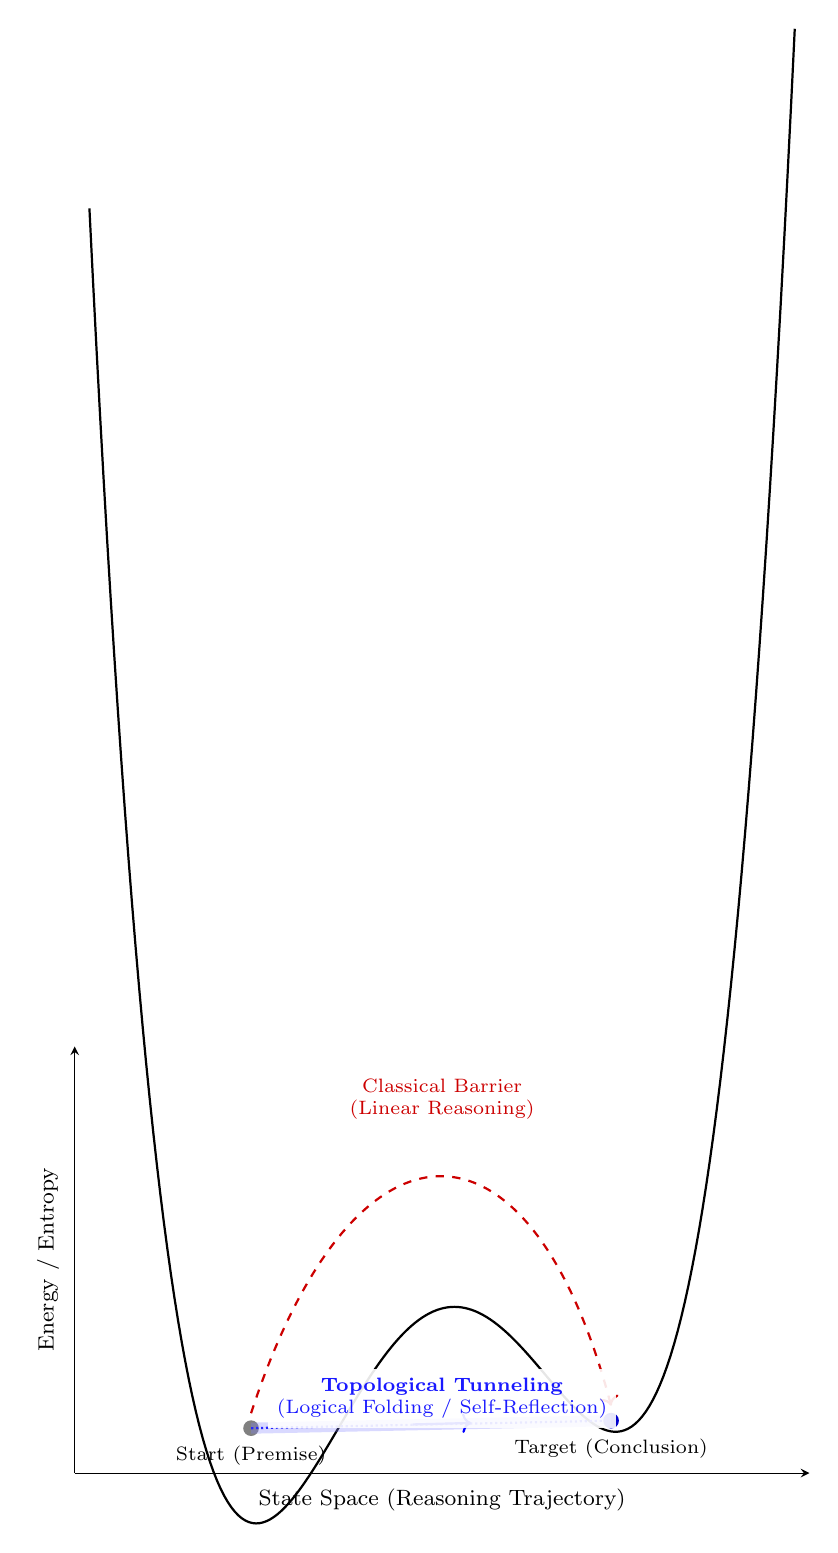
\begin{tikzpicture}
    \begin{axis}[
        width=0.9\textwidth,
        height=7cm,
        axis lines=left,
        xlabel={State Space (Reasoning Trajectory)},
        ylabel={Energy / Entropy},
        xmin=-2.5, xmax=2.5, ymin=-2.2, ymax=3.5,
        xtick=\empty, ytick=\empty,
        label style={font=\footnotesize},
        clip=false
    ]
    % Potential Energy Landscape (Double Well)
    \addplot [domain=-2.4:2.4, samples=200, thick, black] {x^4 - 3*x^2 + 0.5*x};
    
    % Points
    \node[circle, fill=gray, inner sep=2pt, label={[font=\scriptsize]below:{Start (Premise)}}] (start) at (axis cs:-1.3, -1.6) {};
    \node[circle, fill=blue!80!black, inner sep=2pt, label={[font=\scriptsize]below:{Target (Conclusion)}}] (end) at (axis cs:1.15, -1.5) {};
    
    % Classical Path (Sequential)
    \draw[red!80!black, dashed, thick, ->] (axis cs:-1.3, -1.4) .. controls (axis cs:-0.6, 2.8) and (axis cs:0.6, 2.8) .. (axis cs:1.15, -1.3);
    \node[red!80!black, font=\scriptsize, align=center] at (axis cs:0, 2.8) {Classical Barrier \\ (Linear Reasoning)};
    
    % Tunneling Path (Folding/Quantum)
    \draw[blue, thick, densely dotted] (axis cs:-1.3, -1.6) -- (axis cs:1.15, -1.5);
    \draw[blue!50, line width=4pt, opacity=0.3] (axis cs:-1.3, -1.6) -- (axis cs:1.15, -1.5);
    \draw[blue, thick, ->] (axis cs:-0.2, -1.55) -- (axis cs:0.2, -1.53);
    \node[blue, font=\scriptsize, align=center, fill=white, opacity=0.9] at (axis cs:0, -1.2) {\textbf{Topological Tunneling} \\ (Logical Folding / Self-Reflection)};
    \end{axis}
\end{tikzpicture}
\caption{Visualization of Topological Advantage: Classical paths must climb over energy barriers (brute-force linear chain), while topological tunneling (isomorphic to logical folding) enables direct navigation via cluster-state correlations, effectively shortcutting the reasoning space.}
\label{fig:tunneling}
\end{figure}

% --- DISCUSSION ---
\section{Discussion: The Topological Convergence}

\subsection{Contextuality and Non-locality as Computational Resources}
Why do classical machines exhibit quantum-like efficacy? We argue that the \textbf{Attention Mechanism} in Transformers is a classical simulation of quantum \textbf{Non-locality}. In a quantum system, non-locality allows instant correlation regardless of distance. Similarly, Self-Attention allows a token to "attend" to any other token in the sequence immediately, creating a context-dependent reality analogous to quantum \textbf{Contextuality} (where measurement outcomes depend on the context of other measurements).

\subsection{Emergent Quantum-Inspired Algorithms}
The "Folding" observed in Long CoT functions as an emergent \textbf{Quantum-Inspired Algorithm}. Much like Simulated Annealing uses thermal fluctuations to escape local minima on classical hardware, the semantic "van der Waals" forces in AI allow the reasoning trajectory to explore the energy landscape stochastically before collapsing into a low-energy (high-coherence) solution. CAPM formalizes this by mapping these semantic forces to cluster state measurements \cite{raussendorf2001}.

% --- CONCLUSION ---
\section{Conclusion}
The convergence of AI reasoning manifolds and quantum correlation structures signals the dawn of a topological paradigm. By acknowledging that LLMs function as effective quantum simulators via Tensor Networks and Attention-based non-locality, we offer a path out of the brute-force linearity trap. The isomorphism presented here suggests that the next generation of intelligent systems will be characterized not by their computational depth, but by their topological resonance.

% --- BIBLIOGRAPHY ---
\begin{thebibliography}{99}

\bibitem{chen2026}
Chen, Q., Du, Y., Li, Z., et al. (2026). The Molecular Structure of Thought: Mapping the Topology of Long Chain-of-Thought Reasoning. \textit{arXiv preprint arXiv:2601.06002v2}.

\bibitem{nielsen2010}
Nielsen, M. A., \& Chuang, I. L. (2010). \textit{Quantum Computation and Quantum Information} (10th Anniversary Edition). Cambridge University Press.

\bibitem{levine2021}
Levine, Y., et al. (2021). Bridging Many-Body Quantum Physics and Deep Learning via Tensor Networks. \textit{Physical Review Letters}, 127, 141602. (Also: arXiv:2103.06872)

\bibitem{gao2022}
Gao, X., et al. (2022). Transformers as Quantum Circuits: The Role of Tensor Networks in Large Language Models. \textit{arXiv preprint arXiv:2205.14324}.

\bibitem{raussendorf2001}
Raussendorf, R., \& Briegel, H. J. (2001). A one-way quantum computer. \textit{Physical Review Letters}, 86(22), 5188--5191.

\bibitem{briegel2009}
Briegel, H. J., et al. (2009). Measurement-based quantum computation. \textit{Nature Physics}, 5(1), 19--26.

\end{thebibliography}

\end{document}